\documentclass[12pt]{report}
\usepackage{graphicx}                                   %% This package adds graphic options
\usepackage{subcaption}                                 %% This package modifies caption layout
\usepackage{threeparttable}                             %% This package modifies figure spacing
\usepackage{tikz}                                       %% This figure allows the IHG logo on title page
\usepackage{booktabs}                                   %% This package is for tables
\usepackage[export]{adjustbox}                          %% This package aligns photos within a table
\usepackage{array}                                      %% This package allows for customizing tables
\usepackage{rotating}                                   %% This package is for rotating tables
\usepackage{colortbl}                                   %% This package adds color to tables
\usepackage{fancyhdr}                                   %% This package adds fancy headers
\usepackage{multirow}                                   %% This package adds combined rows to tables
\usepackage{xcolor}                                     %% This package adds colors to the document
\usepackage{sectsty}                                    %% This package modifies chapters and sections
\usepackage[titles]{tocloft}                            %% This package modifies TOC layout
\usepackage[a4paper,margin=2.5cm,bottom=2cm]{geometry}  %% This package describes page layout
\usepackage{setspace}                                   %% This package is for line spacing
\usepackage{titlesec}                                   %% This package modifies section titles
\usepackage{enumerate}                                  %% This package is for numbered lists
\usepackage{siunitx}                                    %% This package is for SI unit abreviations
\usepackage[version=4]{mhchem}                          %% This package is for typing chemical components
\usepackage[backend=biber,style=apa,sortcites=yes]{biblatex}    %% This package is for refernces, APA, Sorting


\DeclareFieldFormat[article]{journaltitle}{#1}          %% Removes italics from bibliography
\DeclareFieldFormat[article]{volume}{#1}                %% Removes italics from bibliography
\DeclareFieldFormat[inbook]{booktitle}{#1}              %% Removes italics from bibliography
\DeclareFieldFormat[manual]{title}{#1}                  %% Removes italics from bibliography
\DeclareFieldFormat[report]{title}{#1}                  %% Removes italics from bibliography

\DeclareLanguageMapping{english}{english-apa}           %% Set the cites to APA english style
\addbibresource{sections/references.bib}                %% Add the bibilograph document

%% -------------------------------BELOW this for full citations hyperlinks--------------------------%%
%% -------------------------------BELOW this for full citations hyperlinks--------------------------%%
\DeclareCiteCommand{\cite}
  {\usebibmacro{prenote}}
  {\usebibmacro{citeindex}%
   \printtext[bibhyperref]{\usebibmacro{cite}}}
  {\multicitedelim}
  {\usebibmacro{postnote}}

\DeclareCiteCommand*{\cite}
  {\usebibmacro{prenote}}
  {\usebibmacro{citeindex}%
   \printtext[bibhyperref]{\usebibmacro{citeyear}}}
  {\multicitedelim}
  {\usebibmacro{postnote}}

\DeclareCiteCommand{\parencite}[\mkbibparens]
  {\usebibmacro{prenote}}
  {\usebibmacro{citeindex}%
    \printtext[bibhyperref]{\usebibmacro{cite}}}
  {\multicitedelim}
  {\usebibmacro{postnote}}

\DeclareCiteCommand*{\parencite}[\mkbibparens]
  {\usebibmacro{prenote}}
  {\usebibmacro{citeindex}%
    \printtext[bibhyperref]{\usebibmacro{citeyear}}}
  {\multicitedelim}
  {\usebibmacro{postnote}}

\DeclareCiteCommand{\parenciteA}[\mkbibparens]
  {\usebibmacro{prenote}}
  {\usebibmacro{citeindex}%
    \printtext[bibhyperref]{\printnames{labelname}, \printdate}}
  {\multicitedelim}
  {\usebibmacro{postnote}}

\DeclareCiteCommand{\footcite}[\mkbibfootnote]
  {\usebibmacro{prenote}}
  {\usebibmacro{citeindex}%
  \printtext[bibhyperref]{ \usebibmacro{cite}}}
  {\multicitedelim}
  {\usebibmacro{postnote}}

\DeclareCiteCommand{\footcitetext}[\mkbibfootnotetext]
  {\usebibmacro{prenote}}
  {\usebibmacro{citeindex}%
   \printtext[bibhyperref]{\usebibmacro{cite}}}
  {\multicitedelim}
  {\usebibmacro{postnote}}

\DeclareCiteCommand{\textcite}
  {\boolfalse{cbx:parens}}
  {\usebibmacro{citeindex}%
   \printtext[bibhyperref]{\usebibmacro{textcite}}}
  {\ifbool{cbx:parens}
     {\bibcloseparen\global\boolfalse{cbx:parens}}
     {}%
   \multicitedelim}
  {\usebibmacro{textcite:postnote}}


\DeclareCiteCommand{\citeauthor}
    {}
    {\bibhyperref{\printnames{labelname}}}
    {\multicitedelim}
    {}

\DeclareCiteCommand{\citeauthoryear}
    {}
    {\bibhyperref{\printnames{labelname} \printdate}}
    {\multicitedelim}
    {}

\DeclareCiteCommand{\citeauthoryearpar}
    {}
    {\bibhyperref{\printnames{labelname} \mkbibparens{\printdate}}}
    {\multicitedelim}
    {}

\DeclareCiteCommand{\citeyearpar}
    {}
    {\mkbibparens{\bibhyperref{\printdate}}}
    {\multicitedelim}
    {}

%% -------------------------------ABOVE this for full citations--------------------------%%
%% -------------------------------ABOVE this for full citations--------------------------%%


\usepackage{hyperref}                           %% Package is for hyperlinking refrences
\usepackage[nameinlink,capitalize]{cleveref}    %% Package for refrences,links entire name, capitalized "Fig."




%%===============================================PAGE SETUP==========================================================
  \hypersetup{                                %% Sets hyperlink style,
    colorlinks  =   true,                       %% All links are colored
    urlcolor    =   blue,                       %% DOI color is blue
    linkcolor   =   blue,                       %% Set link color
    linktoc     =   page,                       %% Only the TOC page numbers are linked "all"=page and title
    citecolor   =   blue}                       %% Set cite color

  \captionsetup{                              %% Sets format of figure and table captions
    labelsep        = period,                   %% Period label seperator
    skip            = 3pt,                      %% Sets the gap space between the figure and caption
    font            = {small,sf},               %% Small text, sans serif font
    labelfont       = bf,                       %% Fig and Table are bolded
    singlelinecheck = false}                    %% Single line check

  \captionsetup[sub]{                         %% Sets format of figure and table  SUBcaptions
    font            = {footnotesize,sf},        %% Smaller text, sans serif font
%    labelfont       = normalfont,              %% Subcaption labels are normal font
    singlelinecheck = false}                    %% Single line check


\pagestyle{fancy}                           %% Sets up the headers and footers
    \fancyhead{}                                    %% clear all header fields
    \lhead{                                         %% Format the left header
      \fontsize{10}{12}\selectfont                  %% Font size
      \textcolor{gray}                                                  %% Text color
      {\bfseries Aquatic Habitat Modeling}}         %% Bold font

%% Section title spacing
    \titlespacing*{\section}{0pt}{\baselineskip}{0\baselineskip}        %% No indent, 1 line above, 0 lines below
    \titlespacing*{\subsection}{0pt}{0\baselineskip}{0\baselineskip}    %% No indent, 0 lines above, 0 lines below
    \titlespacing*{\subsubsection}{0pt}{0\baselineskip}{0\baselineskip} %% No indent, 0 lines above, 0 lines below

%% Table set up
    \newcolumntype{B}[1]{>{\centering\arraybackslash}b{#1}}    %% Table paragraph collumn that is centered on the bottom
    \newcolumntype{R}[1]{>{\raggedleft\arraybackslash}b{#1}}   %% Table paragraph collumn that is right aligned on the bottom


%%================================================END PAGE SETUP============================================




%%=============================================BEGIN DOCUMENT===============================================

\begin{document}                            %% Begin the report document

    \onehalfspacing                                               %% Sets 1.5 line spacing

    \setlength{\parskip}{.4\baselineskip}%                        %% Sets the spacing between paragraphs
    \setlength{\parindent}{0pt}%                                  %% Removes the indents from paragaphs
    \renewcommand{\thesection}{\arabic{section}}                  %% Removes chapter number from headings

%%-----------------TITLE PAGE
  \begin{titlepage}

\begin{tikzpicture}[remember picture,overlay]                             %% Insert BOKU logo in upper right, .75cm margin
   \node[anchor=north east,inner sep=.75cm] at (current page.north east)
              {
\includegraphics[width=0.3\linewidth]{images/IHG}};         %% Color photo
\end{tikzpicture}

\begin{center}                                          %% Begin centering all the text
    \vspace*{3cm}                                           %% Insert vertical space

%%----------TITLE
    \LARGE                                                  %% LARGE text for the title
    \textbf{{Report}}

%%----------SUBTITLE
    \vspace{0.5cm}                                          %% Insert vertical space
    %Thesis Subtitle

    \vspace{1.5cm}                                          %% Insert vertical space

%%----------AUTHORS
    \Large                                                  %% Large text for the authos, class and date
    
    
    Jay Morgan - 11729236\\
    Laura Becker - 01169357\\
    Benji Berntatz - 01060697\\
    Leonard Sonten - 01653792\\
    Emily Seiberl - 01008230\\
    \vspace{3cm}                                            %% Insert vertical space

%%----------CLASS
    812381 Aquatic Habitat Modelling
    \vspace{.5cm}                                           %% Insert vertical space

%%----------DATE
    \today                                                  %% Insert today's date
    \vfill                                                  %% Fill the rest of the verticle space

    \end{center}                                            %% End centering of the text

%%----------INSTITUTE
    \normalsize                                             %% Normalesize text for the BOKU info
    Institute of Hydrobiology and Aquatic Ecosystem Management\\
    Department of Water, Atmosphere and Envrionment\\
    BOKU - University of Natural Resources and Life Sciences, Vienna\\





\end{titlepage}

                            %% Clears page and adds title page then clears page


%%-----------------ABSTRACT
    \onehalfspacing                                         %% Sets 1.5 line spacing
    \pagenumbering{roman}                                   %% Sets page number to roman numeral
    \fancyfoot{}                                            %% clear all footer fields (Hide page numbers)

  
\setcounter{secnumdepth}{0}                    %% Removes section number

\section{Abstract}
Abstract about the project                              %% Clears page and adds abstract page then clears page


%%----------------TABLE OF CONTENTS
    \onehalfspacing                                               %% Sets 1.5 line spacing
    \phantomsection                                                 %% Phantom section so TOC links here
  \let\chapter\section\tableofcontents                            %% Insert TOC as a section
      \renewcommand{\cftsecfont}{\fontseries{b}\selectfont}         %% Set TOC sections to bold
      \addcontentsline{toc}{section}{Table of contents}             %% Add TOC to table of contents page


%%----------BODY
    \cleardoublepage                                        %% Reset page numbering
    \pagenumbering{arabic}                                  %% Page number in arabic
    \cfoot{\thepage}                                        %% Adds page numbers to footer

    \onehalfspacing                                         %% Sets 1.5 line spacing
    \setcounter{secnumdepth}{3}                             %% Adds sub-subsection number
%  

\section{Introduction}\label{sec:introduction}                                                   %% The first section

Limited access to clean water has become an increasingly alarming concern around the world. This is not the current situation in Austria, where most of the rivers have low levels of organic pollution. However, through the pursuit of hydropower production and flood protection, Austria’s water bodies face other anthropogenic pressures such as channelization, impoundment and hydropeaking~\parenciteA{Muhar2000}. The EU Water Framework Directive 2000/60/EC (WFD) established the legal obligation of member countries to maintain healthy water resources and mitigate damages inflicted upon their water bodies. The WFD describes a water body’s status by both abiotic and biotic criteria. Biological quality elements are subdivided into assessment of benthic invertebrates, fish, algae and aquatic flora. The ecological status of a water body is defined by comparing the biological community composition present with the near-natural reference conditions. The ecological status is calculated from the residual between the observed condition and the reference condition~\parenciteA{Furhacker2008}.

Benthic invertebrate organisms live in a diverse range of habitats representing a wide variety of aquatic ecosystems. Community structure of MZB responds to environmental disturbances in a rather predictable way. This makes them an excellent candidate for monitoring changes in environmental conditions~\parenciteA{Li2010}. Macrozoobenthos (MZB) are able to reflect different anthropogenic pressures through changes in structure or function of the assemblages. These changes allow for an overall assessment of streams. Aside from organic pollution, MZB can detect habitat loss and overall stream degradation~\parenciteA{Hering2004, Hering2006}. According to~\textcite{Marzin2012}, macroinvertebrate metrics appear to be more sensitive to the degradation of the overall condition of the river than fish metrics. This could be explained by the localized nature of MZB. The insect order Tricoptera are particularly well suited as a bioindicators for describing habitat degradation~\parenciteA{Schmidt-Kloiber2017}.

Many benthic invertebrate species have adapted to specific habitat parameters by way of flow velocity preference, structural needs, feeding strategies and tolerance to pollution~\parenciteA{Stoll2016}. It has been shown that substrate size is one of the best predictors of benthic invertebrate distribution within a river by~\textcite{Jowett2003} and~\textcite{Schroder2013}; while~\textcite{Dohet2015} described the influence that thermal regime and land use has on MZB inhabiting headwater streams. A study of species diversity and functional feeding groups of benthic invertebrates in Austrian rivers, which was carried out by~\citeauthoryearpar{Yoshimura2006}, showed that MZB communities are dependent on their environmental conditions. Studies in Poland have shown that benthic communities have significantly reduced taxonomic richness in constrained channels~\parenciteA{Wyzga2014}.

\begin{figure}[!htb]                                                       %% Reference site photo
  \center
  %\includegraphics[width=.95\linewidth]{images/site_reference}                       %% Width, Image file BW
  \includegraphics[width=.95\linewidth]{images/site_reference_color}                 %% Width, Image file COLOR
  \caption{Reference sample location on Ois River.}                            %% Figure Caption
  \label{fig:site_reference}                                                        %% Figure label key
\end{figure}


This report focuses on the benthic invertebrate communities sampled from two Alpine rivers near Lunz-am-see. We collected and assessed a sample of the benthic community from a near-natural site of the Ois River~(\cref{fig:site_reference}). This was to be used as a reference site when compared to a sample which was collected from a heavily impacted site of the Maiergraben. By comparing the collecting samples from the Ois and Maiergraben, we hope to answer the following questions:

\singlespacing                                              %% Set single spacing
\begin{enumerate}
  \item Does habitat availability differ between the unimpacted Ois River and the impacted Maiergraben?
  \item Is there a relation between choriotope and sensitive screening taxa?
  \item What influence do microhabitats have on benthic communities within a river?
  \item Is there a difference in taxa composition, diversity and abundance between the unimpacted Ois and impacted Maiergraben?
  \item Does the benthic community represent the observed impacts at the Maiergraben?
\end{enumerate}
\onehalfspacing                                             %% Sets 1.5 line spacing


We hypothesized that the hydro-morphologically dynamic Ois River will contain more diverse habitat than the constrained Maiergraben. We predicted that some screening taxon are associated with specific choriotopes. We also hypothesized that habitat heterogeneity will result in more taxon richness and abundance, with an increase in specialized taxa. We predicted that the taxa composition, diversity and abundance would differ between the two sites, with the Ois River having a higher diversity and abundance than the Maiergraben. We assumed that the benthic community of the Maiergraben will be comprised of taxon associated with heavily impacted and channelized rivers.

                                   %% Adds introduction to report
%  

\section{Materials and Methods}\label{sec:material_methods}          %% The first section

\subsection{Study area}\label{sec:study_area}                %% The Study areas




The benthic macro-invertebrate samples were taken at two sites near lake Lunz (Mostviertel, lower Ausrtria). For reference conditions the Ois River in Lunz am See was sampled~(\cref{fig:site_reference}). This small, natural, alpine river represents the headwaters of the Ybbs River and subsequently flows into the Danube river. The second sampling site was the so called Maiergraben, a small, concreted, channelized creek flowing through a forested area into lake Lunz~(\cref{fig:site_impactedA}).



\begin{figure}[!htb]                                                        %% Impacted site photo
	\centering                                                                  %% Center the figures
	\subcaptionbox{Heavy regulation present at impacted site.\label{fig:site_impactedA}}{   %% First subcaption
		%\includegraphics[width=0.48\columnwidth]{images/site_impacted1}}         %% Set width and select first image BW
		\includegraphics[width=0.48\columnwidth]{images/site_impacted1_color}}    %% Set width and select first image COLOR
	\hfill                                                                                    %% Fill Blank space
	\subcaptionbox{Sample collection from impacted area.\label{fig:site_impactedB}}{        %% Second subcaption
		%\includegraphics[width=0.48\columnwidth]{images/site_impacted2}}              %% Set width and second image BW
		\includegraphics[width=0.48\columnwidth]{images/site_impacted2_color}}        %% Set width and second image COLOR
	\hspace*{\fill}                                                                           %% Fill blank space
	\caption{Impacted site located on Maiergraben.}\label{fig:site_impacted}          %% Capition for both figures
\end{figure}




\subsection{Methods}\label{sec:methods}                         %% The methods section

\subsubsection{Multi-Habitat Sampling (MHS)}\label{sec:mhs}         %% Describe MHS


For this approach the examined river reach was partitioned into 20 subunits. These sampling units were representing different habitat types (choriotopes) and their proportional areal coverage within the reach. Sampling units were characterized by both mineral~(\cref{tab:choriotope_mineral}) and biotic~(\cref{tab:choriotope_biotic}) habitats.


\begin{table}[!htb]                                 %% Mineral choriotope table
  \small                                                       %%makes the table font small
  \centering
  \caption{Mineral choriotopes.}
    \begin{tabular}{ l l p{7cm} }
  \toprule
    Nomenclature  &
    \multicolumn{1}{c}{Grain size}  &
    \multicolumn{1}{c}{Description of choriotope} \\
  \hline
  \hline
    megalithal      & \textgreater 40 cm               & upper sides of boulders, large cobbles and blocks, bedrock\\
    macrolithal     & \textgreater 20 cm to 40 cm      & coarse blocks, head-sized cobbles, variable percentages of cobbles, gravel and sand\\
    mesolithal      & \textgreater 6.3 cm to 20 cm     & fist to hand-sized cobbles and pebbles with a variable percentage of gravel and sand\\
    microlithal     & \textgreater 2 cm to 6.3 cm      & pebbles, coarse gravel with percentages of medium to fine gravel\\
    akal            & \textgreater 0.2 cm to 2 cm      & fine to medium-sized gravel\\
    psammal         & 0.063 mm to 2 mm      & sand\\
    pelal           & \textless 0.063 mm            & mud and sludge\\
    argillal        &                       & silt, loam and clay\\
  \bottomrule
    \end{tabular}
  \label{tab:choriotope_mineral}%
\end{table}%


First the share of mineral habitat classes was defined, secondly the biotic habitats within the mineral habitats were classified. This was done by a visual estimation of the area. For every 5\% of a certain choriotope (combination of mineral and biotic habitat) one sampling unit was chosen. The shares and subunits of each choriotope were then put in a field-protocol~(see~\hyperref[appendixA]{Appendix A}).

Sampling units also had to be distributed accordingly between the mesohabitats (river bottom/bank, lentic/lotic, riffles/pools). As the sampling area should not be disturbed beforehand, the sampling started downstream and then proceeded upstream.


%\paragraph{Habitat Composition}\label{sec:choriotopes}         %% Describe chiriotopes



\begin{table}[!htb]                                 %% Biotic choriotope table
  \centering
  \small                                                       %%makes the table font small
  \caption{Biotic choriotopes.}
    \begin{tabular}{ l l }
  \toprule
    Nomenclature  &
    \multicolumn{1}{c}{Description of choriotope} \\
  \hline
  \hline
    algal periphyton    & areal stone cover\\
    filamentous algae   & tufts or floating mats\\
    mosses              & -\\
    macrophytes         & submerged plants\\
    living wood         & roots, branches (with leaves),\newline tree trunks\\
    deadwood            & branches and tree trunks\\
    CPOM                & course particulate matter\\
    FPOM                & fine particulate organic matter\\
    sapropel            & decaying sludge\\
    bacteria \& fungi   & lawns and tufts\\
  \bottomrule
    \end{tabular}
  \label{tab:choriotope_biotic}%
\end{table}%










\subsubsection{Sampling Method}\label{sec:sampling_method}          %% Describe impacted site

\begin{table}[!htb]                                         %% Ois Choriotopw Table
  \small                                                       %%makes the table font small
%  \centering
  \caption{Choriotope description of the sampling units at the Ois River.}
  \resizebox{\textwidth}{!}{                                                          %% Resizes the table to the text
  \begin{tabular}{ r b{.12\textwidth} b{.15\textwidth} c r r r }
    \toprule
    \multicolumn{1}{R{.08\textwidth}}{Sample} &
    \multicolumn{1}{B{.13\textwidth}}{Mineral Habitat} &
    \multicolumn{1}{B{.17\textwidth}}{Biotic \par\noindent Habitat} &
    \multicolumn{1}{B{.15\textwidth}}{Velocity \par\noindent [m/s]} &
    \multicolumn{1}{B{.08\textwidth}}{Velocity Class} &
    \multicolumn{1}{B{.08\textwidth}}{Water Depth \par\noindent [cm]} &
    \multicolumn{1}{B{.1\textwidth}}{Distance \par\noindent to Shore\par\noindent [m]} \\
    \hline
    \hline
    1\_2 & mesolithal & micro\_algae & 0.9   & high  & 10    & 2 \\
    3\_4 & macrolithal & micro\_algae\_moss & 1.3   & very\_high & 25    & 6 \\
    5\_6 & megalithal & moss  & 1.3   & very\_high & 5     & 8 \\
    7\_8 & mesolithal & micro\_algae & 0.5   & medium & 20    & 4 \\
    9\_10 & megalithal & micro\_algae & 0.5   & medium & 10    & 8 \\
    11\_12 & mesolithal & periphyton & 0.2   & slow  & 30    & 5 \\
    13\_14 & akal & none  & 0.2   & slow  & 25    & 2 \\
    15\_16 & mesolithal & CPOM  & {  0}     & no\_flow & 20    & 0.5-1 \\
    17\_18 & macrolithal & micro\_algae & {  0}     & no\_flow & 10    & 0.5 \\
    19\_20 & mesolithal & CPOM  & 0.2   & slow  & 20    & 0.5 \\
    \bottomrule
    \end{tabular}}%
  \label{tab:choriotope_ois}%
\end{table}%



Sample collection at each sampling unit was performed with a stationary rectangular net (Mesh size: \SI{500}{\micro\meter} EU standard) and by disturbing a quadratic area upstream of the net (25x25cm). For the Ois River we chose 10 sampling locations where we took 2 samples each, for a total of 20 units~(\cref{tab:choriotope_ois}).




Since the Maiergraben had a very homogenous structure we chose only four sampling locations – three in the creek and one under a small bridge. We collected 5 samples from each location for a total of 20 sampling units.~(\cref{tab:choriotope_maiergraben,fig:site_impactedB})


\begin{table}[!htb]
  \small                                                       %%makes the table font small
  %\centering
  \caption{Choriotope description of the sampling units at the Maiergraben.}
  \resizebox{\textwidth}{!}{                                                          %% Resizes the table to the text
  \begin{tabular}{ r b{.12\textwidth} b{.18\textwidth} c r r r }
    \toprule
    \multicolumn{1}{R{.08\textwidth}}{Sample} &
    \multicolumn{1}{B{.13\textwidth}}{Mineral Habitat} &
    \multicolumn{1}{B{.17\textwidth}}{Biotic \par\noindent Habitat} &
    \multicolumn{1}{B{.15\textwidth}}{Velocity \par\noindent [m/s]} &
    \multicolumn{1}{B{.08\textwidth}}{Velocity Class} &
    \multicolumn{1}{B{.08\textwidth}}{Water Depth \par\noindent [cm]} &
    \multicolumn{1}{B{.1\textwidth}}{Distance \par\noindent to Shore\par\noindent [m]} \\
    \hline
    \hline
    1-5   & technomega & micro\_macro\_algae & 0.22-0.32 & medium & 4.8   & 0.5 \\
    6-10  & technomega & micro\_macro\_algae & 0.24-0.34 & medium & 2.8   & 0.5 \\
    11-15 & technomega & micro\_macro\_algae & 0.22-0.32 & medium & 4.5   & 0.5 \\
    16-20 & technomega & bare  & 0.30-0.40 & medium & 4.2   & 0.5 \\
    \bottomrule
    \end{tabular}}%
  \label{tab:choriotope_maiergraben}%
\end{table}%


Samples taken from organic habitats, always had to include the underlying mineral substrates. The different mineral habitats needed to be sampled accordingly.
\begin{list}{}
  \item {\textbf{Megalithal:} Boulders were sampled from all sides by sweeping the surface with a brush and flushing the animals into the net.}
  \item {\textbf{Macro- and Mesolithal:} Surface dwelling animals were flushed in the net by gently sweeping the cobbles or stones by hand. Next clingers and sessile animals were scratched off with a brush. Finally, the underlying substrate (within 15 to 20 cm depth) was churned by foot.}
  \item {\textbf{Microlithal and Akal:} Coarse gravel and sandy substrate was sampled by disturbing the sediment by kicking it downstream the net.}
\end{list}

After sampling each unit, the content of the net was transferred first into a tray and then into a closable bucket, which was filled with ethanol, in order to kill the animals.


\subsubsection{Sorting Techniques}\label{sec:sorting_technigues}      %% Describe impacted site

To sort the animals by size classes the buckets contents were later put through a sieve tower with different mesh sizes (\SI{10}{\milli\meter} down to \SI{500}{\micro\meter}). The different fractions were then placed in trays~(\cref{fig:sorting_tray}), so animals could be sorted, counted and determined to screening taxa level with the help of binoculars~(\cref{fig:sorting}). Only whole animals, so no single body parts, empty shells, exuvies or headless animals were taken into account. In trays with large amounts of animals (usually the smaller fractions) rare or single-occurring animals were taken out, and the rest was subsampled. This was done by transferring the animals in another tray that consisted of a grid, separating the tray into 16 or 8 cells. The organisms of usually two representing subsamples were determined and counted. The number of animals then had to be multiplied accordingly.
A taxa list was created with MS Excel and further analysis were made with the programs MS Excel and EcoProf (version 4.0.0).






\begin{figure}[!htb]                               %% Sample processing
\centering                                                                  %% Center the figures
\captionbox{Sorting tray used for taxa identification.\label{fig:sorting_tray}}{   %% First subcaption
  %\includegraphics[height=7.6cm]{images/sorting_tray}}               %% Set width and select first image BW
  \includegraphics[height=7.6cm]{images/sorting_tray_color}}         %% Set width and select first image COLOR
  \hfill                                                                                    %% Fill Blank space
\captionbox{Identifying taxa within the samples using binoculars.\label{fig:sorting}}{     %% Second subcaption
  %\includegraphics[height=7.6cm]{images/sorting}}              %% Set width and second image BW
  \includegraphics[height=7.6cm]{images/sorting_color}}        %% Set width and second image COLOR
  \hspace*{\fill}                                                                    %% Fill blank space
\end{figure}




\subsection{Equipment}\label{sec:equipment}                 %% The equipment section


\begin{table}[htbp]
  \centering
    \begin{tabular}{l b{3cm} l}
    ·         Nets & ·   &      Sieve tower \\
                &   &\\
    ·         Brushes & · &        Sorting trays~(\cref{fig:sorting_tray}) \\
                &   &\\
    ·         Trays & ·    &     Subsampling trays \\
                &   &\\
    ·         Buckets (closeable) & ·  &       Tweezers \\
                &   &\\
    ·         Ethanol & ·     &    Binoculars \\
    \end{tabular}%
  \label{tab:addlabel}%
\end{table}%


                                        %% Adds methods to report
  
\section{Results}\label{sec:results}                           %% The first section





\subsection{River2D Modelling}\label{sec:river2d}       




The software program River2D was used to calculate the habitat suitability in a section of the River Ybbs. First a model was created of the River Ybbs. A file containing habitat suitability parameters of brown trout at different age classes was prepared. Choriope information was also entered into River2D. The software then calculated the weighted usable area (WUA) for the age classes at different flow rates (\SI[per-mode=symbol]{0.35}{\cubic\meter\per\second} - \SI[per-mode=symbol]{2.16}{\cubic\meter\per\second} - \SI[per-mode=symbol]{6.00}{\cubic\meter\per\second} - \SI[per-mode=symbol]{13.00}{\cubic\meter\per\second} - \SI[per-mode=symbol]{20.00}{\cubic\meter\per\second}). \cref{fig:flow_rate_age_class} shows the total WUA of age classes at each flow rate. The 0+ fish have a much higher WUA at low flows, while the larger 2+ fish have almost no WUA at \SI[per-mode=symbol]{0.35}{\cubic\meter\per\second} flow.


\begin{figure}[!htb] 
	\centering
	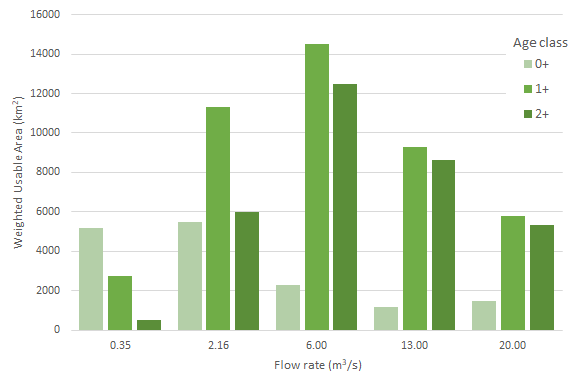
\includegraphics[width=.8\textwidth]{images/flow_rate_age_class}
	\caption{Total weighted usable area by age class and flow rate in the River Ybbs for brown trout as calculated by River2D.}\label{fig:flow_rate_age_class}
\end{figure}

River2D was then used to create maps of the Ybbs showing the combined suitabilty for each age class. At \SI[per-mode=symbol]{0.35}{\cubic\meter\per\second}, adult brown trout have very limited habitat available, thus habitat suitability is very low (\cref{fig:2_0035}). Conversely, \cref{fig:2_0600} shows that a flow rate of \SI[per-mode=symbol]{6.00}{\cubic\meter\per\second} provides an abundance of habitat and near ideal conditions for adult brown trout. See the~\hyperref[appendixA]{Appendices} for the collection of maps representing the combined suitability of all brown trout age classes at different flow rates. 


\begin{figure}[!htb] 
	\centering
	\begin{subfigure}{.3\textwidth}
		\centering
		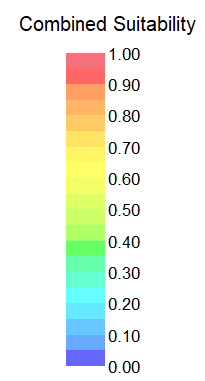
\includegraphics[width=.9\linewidth]{images/suitability_index}
	\end{subfigure}%
	\begin{subfigure}{.7\textwidth}
		\centering
		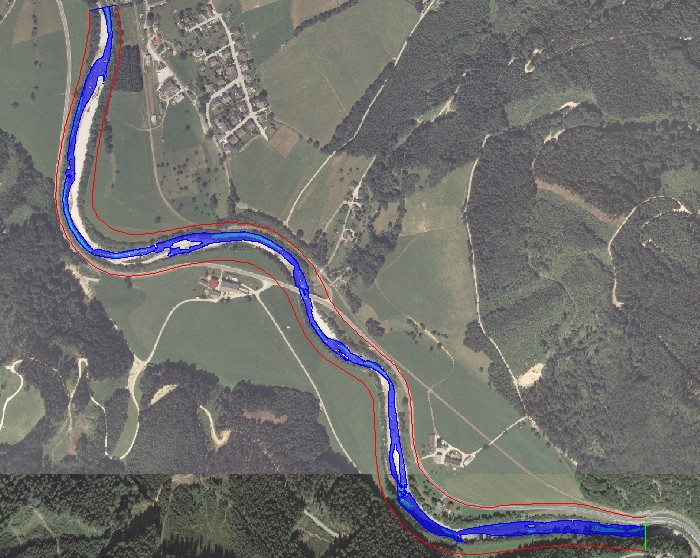
\includegraphics[width=\linewidth]{images/2_0035}
	\end{subfigure}
	\caption{Brown trout (2+ class) combined suitability at \SI[per-mode=symbol]{0.35}{\cubic\meter\per\second}.}
	\label{fig:2_0035}
\end{figure}


\begin{figure}[!htb] 
	\centering
	\begin{subfigure}{.3\textwidth}
		\centering
		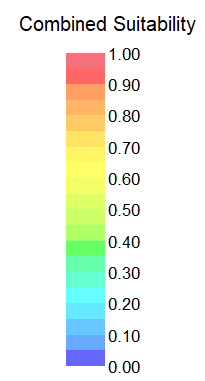
\includegraphics[width=.7\linewidth]{images/suitability_index}
	\end{subfigure}%
	\begin{subfigure}{.7\textwidth}
		\centering
		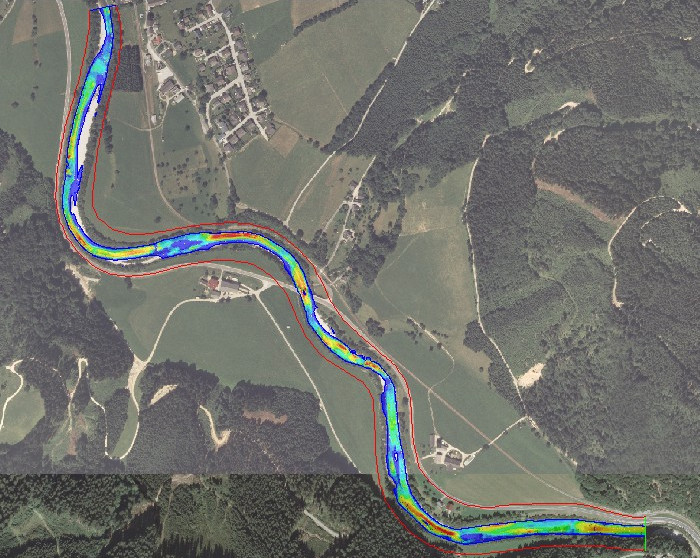
\includegraphics[width=\linewidth]{images/2_0600}
	\end{subfigure}
	\caption{Brown trout (2+ class) combined suitability at \SI[per-mode=symbol]{6.00}{\cubic\meter\per\second}.}
	\label{fig:2_0600}
\end{figure}



\begin{figure}[!htb]                                                        	%% SI depth
	
	\centering                                                                  	%% Center the figures
	\hfill
	\subcaptionbox{Depth SI for 1+\label{fig:SI_depth_1}}{   	%% First subcaption
		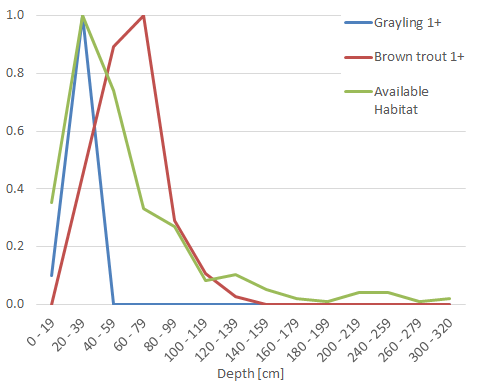
\includegraphics[width=0.48\columnwidth]{images/SI_depth_1}}   						%% Set width and select first image COLOR
	\hfill                                                                   		%% Fill Blank space
	\subcaptionbox{Depth SI for 2+\label{fig:SI_depth_2}}{    %% Second subcaption
		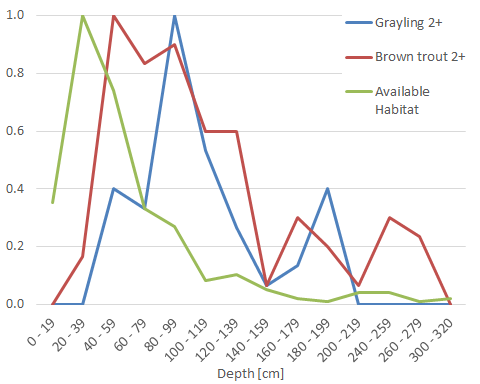
\includegraphics[width=0.48\columnwidth]{images/SI_depth_2}}        				%% Set width and second image COLOR
	\hspace*{\fill}                                                                         %% Fill blank space
	\hfill
	\subcaptionbox{Mean velocity SI for 1+\label{fig:SI_vmean_1}}{   	%% First subcaption
		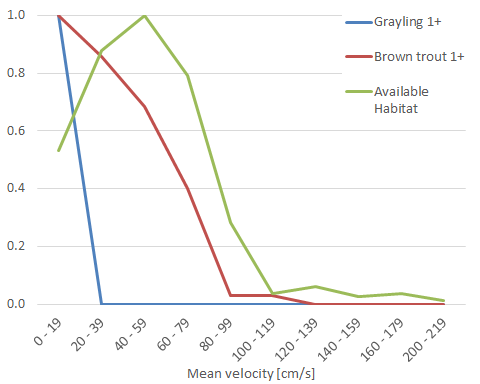
\includegraphics[width=0.48\columnwidth]{images/SI_vmean_1}}   						%% Set width and select first image COLOR
	\hfill                                                                   		%% Fill Blank space
	\subcaptionbox{Mean velocity for 2+\label{fig:SI_vmean_2}}{    %% Second subcaption
		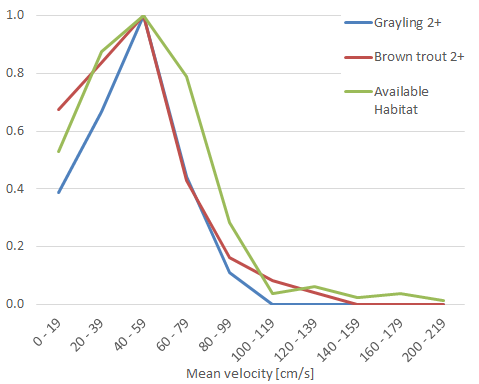
\includegraphics[width=0.48\columnwidth]{images/SI_vmean_2}}        				%% Set width and second image COLOR
	\hspace*{\fill}                                                                         %% Fill blank space
	
	\caption{Calculated habitat suitability index ratings (SI) of different age classes by depth and mean velocity from the sampled area of the Ois River.}\label{fig:SI_depth}        %% Capition for both figures
\end{figure}


























                                        %% Adds results to report
%  

\section{Discussion}\label{sec:discussion}                 %% The first section

In the following part the results of the assessment will be discussed following the same order as in the results section.

\subsection{Microhabitats}\label{sec:disc_microhabitats}       %% The first subsection of discussion


When comparing the two rivers Ois and Maiergraben, the differences between them are quite obvious. The Ois is in a very good ecological status according to both the organic and general degradation. The substrate size of the Ois ranged from sand to megalithal. Together with a broad range of flow velocities and water depths, benthic invertebrate taxa encounter different microhabitats to colonise. meso- and macrolithal together occupy 70\% of the mineral microhabitats, which creates a big surface to colonise with a lot of interstitial space. Furthermore, different biotic cover is present at mesolithal habitats such as micro algae in medium (7\_8) to high flow velocities (1\_2) and periphyton in slow flow velocities (11\_12). At sampling sites with slow flow velocities (19\_20) or no flow (15\_16), aggregations of CPOM are present. The macrolithal contains micro algae/moss at very high flow velocities (3\_4) and micro algae where no flow is present (17\_18). The akal microhabitat has no biotic cover (13\_14), which can be explained by the instability of the substrate, whereas megalithal is covered by either moss (5\_6) or micro algae (9\_10). At the Ois, habitats for various benthic invertebrate taxa with different strategies are available. CPOM supplies grazers with food whereas micro and macro algae, moss and Periphyton support grazers and other animals which cling to plant parts in order to cope with high currents. Low flow velocities provide habitats for swimming animals and others, which are not well adapted to high flow velocities. On the other hand do very high flow velocities support filter feeders, which can be observed at the sampling sites 1\_2 and 3\_4, where simulids occur in high numbers~(\cref{fig:taxa_ois}).


According to the Screening Taxa analysis~(\cref{fig:ecoprof}), the Maiergraben is in a worse ecological status due to general degradation and therefore in need of action. The Maiergraben is framed by a corset of Techno-megalithal (\cref{fig:site_impactedA}), which lowers its habitat heterogeneity at both levels, the abiotic and biotic, when compared to the Ois. Due to steep stone walls at either side as well as at the river bed, the water depth is uniform and therefore formations of sections with lower flow velocity and deeper areas are highly restricted. Additionally, the lateral connectivityt to the floorplain is no longer available. As can be seen in \cref{tab:choriotope_maiergraben}, the flow velocity is very monotonous and classified as medium and therefore CPOM and FPOM can easily be washed out. The good saprobity-status of the Maiergraben underlines this assumption.

The biotic habitat in the Maiergraben is rather monotonous too, whereby 15 out of 20 sampling points are overgrown by micro/macro algae. Clear water and low water depths allow penetration of sunlight through the water column, which makes plant growth possible. The remaining five sites without algal cover were located below a bridge and therefore in the shadow and lay bare.


\subsection{Taxa Composition}\label{sec:disc_taxa_composition}      %% The second section of discussion


The taxa composition of the Ois is diverse with 48 present taxa~(\cref{fig:ecoprof}), which can be explained by its habitat heterogeneity as discussed above. In the following section five different habitats 1\_2, 7\_8, 9\_10, 17\_18 and 19\_20, which differ most in their taxa composition, are discussed.

Sampling site 1\_2 has a high abundance of 1818 Ind./\SI{}{\square\meter} and is dominated by simulids, which are passive filter feeders~\parenciteA{Car2002} and their occurrence can be explained by high flow velocities and algal cover (\cref{tab:choriotope_ois}), which can be used to cling on in order to cope with high currents as seen in~\cref{fig:simulidae}. Dominating ephemeropterans are from the family Baetidae, which are assumed to hide in the micro algae cover or in the interstice of the mesolithal because due to their shape the adaption to high current is not very high. The second dominating ephemeropterans, \emph{Rhithrogena, sp.}, on the other hand are well adapted to high flow velocities and graze on algal cover or feed on detritus, which is trapped between plant parts~\parenciteA{Bauernfeind2002}. Furthermore, occurring plecopterans belong to Capniidae/Leuctridae, \emph{Amphinemura} sp. and \emph{Protonemura} sp., which are classified as grazer, shredders and detrivorous, as well as \emph{Isoperla} sp. and \emph{Dinocras} sp., which are predators.

Sampling site 7\_8 is not dominated by any taxa group and abundance is lower with 706 Ind./\SI{}{\square\meter}. The habitat is characterised by mesolithal and therefore a big surface to colonise, overgrown with micro algae and medium flow velocity (\cref{tab:choriotope_ois}). Ephemeropterans are represented mainly by Baetidae and \emph{Rhithrogena} sp., which are different according to their adaption to high flow velocities. \emph{Rhithrogena} sp. belongs to the family Heptagenidae, which have a characteristically flattened body shape, whereas Baetidae are rather slim. Both taxa are grazers and detritus feeders~\parencite{Bauernfeind2002}. Furthermore, coleopteran are represented by \emph{Elmis} sp. and \emph{Esolus/Oulimius/Riolus} sp., which are grazing, shredding or detrivorous and \emph{Hydraena} sp., which is grazing as an adult while clinging to stones or plant parts with its hooks and predatory as a larvae~\parenciteA{Jach2002}. Plecoptera are represented by the same taxa as at sampling site 1\_2 and show a similar pattern in abundances. Trichopterans are represented by the families Glossosomatidae, Limnephilidae and Sericostomatidae and also a small number of \emph{Brachycentrus montanus}, which is classified as passive filter feeder, as well as predatory and grazing~\parenciteA{Graf2002a}. Additionally, chironomids and other dipterans are present.



\begin{figure}[!htb]                            %% Caddis fly cases
  \center
  %\includegraphics[width=.75\linewidth]{images/simulidae}                   %% Width, Image file BW
  \includegraphics[width=.75\linewidth]{images/simulidae_color}              %% Width, Image file COLOR
  \caption{Mass abundances of Simulidae (black flies) found at Ois river.}            %% Figure Caption
  \label{fig:simulidae}                                                        %% Figure label key
\end{figure}

Sampling site 9\_10 is characterised by megalithal, which is overgrown with micro algae and medium flow velocity (\cref{tab:choriotope_ois}) and is clearly dominated by chironomids. Additionally, higher abundances of \emph{Protonemura} sp., Baetidae Gen. sp. and Elmidae Gen. sp. let assume that accumulations of detritus are available since all taxa are at least partly detritus feeding. At this sampling site together with site 3\_4 trichopterans are most diverse and represented by six taxa, namely Rhyacophilidae Gen. sp, Hydroptilidae Gen. sp., \emph{Hydroptila} sp., \emph{Hydropsyche} sp., Psychomyiidae Gen. sp. and \emph{Micrasema minimum}.

Sampling site 17\_18 has no flow and is characterised by macrolithal and micro algae (\cref{tab:choriotope_ois}). The dominating group are ephemeropterans, mainly due to \emph{Ephemerella} sp., which are grazing and detrivorous~\parenciteA{Bauernfeind2002} and seem to thrive with no flow and growth of micro algae because they account for almost 50\% of all individuals. This site is also the only one where oligochaets are present, represented by \emph{Nais} sp.

The last sampling site to be discussed is site 19\_20, which is characterised by mesolithal, slow flow velocity and CPOM cover (\cref{tab:choriotope_ois}). More than 95\% of occurring taxa belong to the EPT-Taxa; however, the total abundance is lowest with 236 Ind./\SI{}{\square\meter}. Dominating plecopterans are Capniidae/Leuctridae and \emph{Amphinemura} sp., which are classified at least partly as shredders~\parenciteA{Graf2002}. The most dominant ephemeropteran taxa are again \emph{Ephemerella} sp., indicating their preference for little current. \emph{Ecdyonurus} sp. and \emph{Baetis muticus} are occurring too, which are characterised as grazing and detrivorous~\parenciteA{Bauernfeind2002}. Since the water level is low algal cover is present and slow flow velocities together with availability of CPOM encourage formation of detritus. The present trichopterans are Limnephilidae Gen. sp., Sericostomadidae Gen. sp. and \emph{Potamophylax rotundipennis}. The latter one is mainly shredding organic material and to small parts also grazing and predatory.

However, a pattern of lower abundances at sampling sites 13\_14 to 19\_20 (they range between 236-424 Ind./\SI{}{\square\meter}), where flow velocities are either slow or missing, can be observed. A possible explanation can be a lower availability of food items, whereas habitats with higher flow velocities are supplied continuously. At sites where CPOM is available this assumption might not be true. The site 11\_12 is the only one with slow flow velocity and a higher abundance (924 Ind./\SI{}{\square\meter}), but also the only site which is covered with periphyton. The high abundance is due to domination of chironomids (406 Ind./\SI{}{\square\meter}), which seem to be well adapted.

At Maiergraben the taxa composition is rather similar at all sampling sites (\cref{fig:taxa_maiergraben}) and in total only 24 different taxa are present~(\cref{fig:ecoprof}). Interestingly, abundances differ greatly from 182 Ind./\SI{}{\square\meter} at site 16-20 to 2910 Ind./\SI{}{\square\meter} at site 6-10. The site 16-20 is also the only one where no biotic cover is present and therefore an important microhabitat and food source is missing. The dominating group are always chironomids followed by ephemeropterans except at sampling site 6-10, where simulids are the second most abundant group. At site 6-10 chironomids (2011 Ind./\SI{}{\square\meter}) and simulids (464 Ind./\SI{}{\square\meter}) together account for almost 2500 Ind./\SI{}{\square\meter}. A reason for high simulid abundances could be the very low water depth of 2.8 cm (\cref{tab:choriotope_maiergraben}), which makes filtering easy because food is always close. Ephemeropterans are represented by Baetidae Gen. sp. at all sites except of an additional specimen (1 Ind./\SI{}{\square\meter}) of \emph{Rhithrogena} sp. at site 6-10. Trichopterans are more diverse, but most dominant are the taxa Rhyacophilidae Gen. sp., Rhyacophila s. str. Sp. and Rhyacophila aquitanica/tristis, which belong to the predators~\parencite{Graf2002a} and seem to benefit from the high abundances of chironomids. Coleopterans at all sites belong to Esolus/Oulimnius/Riolus sp., which are classified as grazing, shredding and detrivorous~\parencite{Jach2002} and might feed as grazers at the sites 1-15 and as detritus feeders at site 16-20.




\subsection{EPT-Taxa}\label{sec:disc_ept_taxa}                      %% The third section of discussion

The abundance of EPT-Taxa is shown for both the Ois and Maiergraben in \cref{fig:EPT}. In total 29 EPT-Taxa are present at the Ois and 12 at the Maiergraben. Additionally, many more individuals are present at the Ois, which is especially true for plecopterans, where individuals of Capniidae/Leuctridae, \emph{Amphinemura} sp. and \emph{Protonemura} sp. are often among the dominating taxa. The same is not true for the Maiergraben, where abundances of plecopterans are generally low. One possible explanation is the lack of interstices, which are often used by those taxa. Furthermore, those groups show highest abundances at sample sites 3\_4 and 5\_6 with very high flow velocity and the presence of moss. At the Maiergraben no predatory plecopterans are present, but many predatory trichopteran taxa are. Moreover, abundances of trichopterans are very similar at both rivers; however, the taxa are more diverse at the Ois, where 14 taxa are present compared to seven at Maiergraben. This fits to the assumption that in impacted rivers less taxa, but higher abundances occur compared with many taxa and less abundance in intact stretches (compare with~\hyperref[appendixB]{Appendix B} ). The Ois shows higher number of taxa and higher abundances of ephemeropterans too. At the Maiergraben only two taxa are present whereby \emph{Rhithrogena} sp. has an abundance of 1 Ind./\SI{}{\square\meter}. Furthermore, Baetidae Gen. sp. are given a BMWP-Score of only 4, which indicates that they are not very sensitive~\parenciteA{Martin2007}. Even though all flow velocities at Maiergraben are classified as medium only little ephemeropteran taxa, which are adapted to those flow velocities, are present. At the Ois, on the other hand, many different taxa are present with various adaptations to their environment.



\subsection{Sensitive Taxa}\label{sec:disc_sensitive_taxa}          %% The fourth section of discussion

The number of sensitive taxa differs between both rivers. In the Ois 27 taxa are present, whereas in the Maiergraben only six taxa are present, which is one reason for the low score at the general degradation (\cref{fig:ecoprof}). In the Ois 56\% of all taxa are classified as sensitive and 25\% at the Maiergraben (\cref{fig:sensitive}). On average, 12.4 sensitive taxa are present at a site in the Ois and 3.25 at the Maiergraben.

At the Ois the taxa belong to the groups Coleoptera, Diptera, Ephemeroptera, Plecoptera and Trichpotera. Some taxa such as \emph{Amphinemura} sp., \emph{Protonemura} sp., \emph{Rhithrogena} sp., \emph{Ephemerella} sp., \emph{Hydraena} sp., \emph{Elmis} sp. and \emph{Micrasema minimum} show high abundances.

At the Maiergraben the taxa belong to Cleoptera, Diptera, Ephemeroptera and Plecoptera and except for Elmidae Gen. sp. and \emph{Protonemura} sp. abundances are very low.
                                     %% Adds discussion to report

%  

\section{Conclusions?}\label{sec:conclusion}                                                   %% The first section

\subsection{Subsection needed?}\label{XXXXXXXXXXXXXXXXXXXXXXXX}       %% The first subsection of first section

                                     %% Adds conclusion to report

    \clearpage                                                  %% Clears page before References


%%------------REFERENCES and APPENDIX


    \onehalfspacing                                                 %% Sets 1.5 line spacing
    \fancyfoot{}                                                    %% clear all footer fields (Hide page numbers)
    \nocite{*}                                                      %% List references even if uncited
    \printbibliography[title=References,heading=subbibnumbered]     %% Add bibliography, Change title, Number Section

  

%%================================================= PAGE SETUP==============================================
    \renewcommand{\thesubsection}{\Alph{subsection}}                  %% Removes section number from subsection appendix

    \newcommand{\fakesection}[1]{%                          %% Creates a fake section for the TOC
      \par\refstepcounter{section}                               %% Increase section counter
      \sectionmark{#1}                                           %% Add section mark (header)
      \addcontentsline{toc}{section}{#1}}                         %% Add section to ToC

    \newcommand{\fakesubsection}[1]{%                                       %% Creates a fake subsection for the TOC
      \par\refstepcounter{subsection}                                         %% Increase section counter
      \sectionmark{#1}                                                           %% Add section mark (header)
      \addcontentsline{toc}{subsection}{\protect\numberline{\thesubsection}#1}}  %% Add subsection to ToC

    \titleformat{\subsection}                               %% Centering of the Appendix Titles
      {\large\bfseries\centering}
      {\thesection}{}{}
%%================================================END PAGE SETUP============================================



\fakesection{Appendices}                               %% Adds section to TOC but not the page


%%----------------Appendix A
\fakesubsection{\SI[per-mode=symbol]{0.35}{\cubic\meter\per\second} flow rate models} %% Adds subsection to TOC but not the page
\subsection*{Appendix A}\label{appendixA}                        %% Adds subsection to page but not the TOC

\renewcommand\thefigure{A.\arabic{figure}}                          %% Begins numbering the appendix figures with A
\setcounter{figure}{0}                                              %% Restarts the figure counter

\centering
\begin{figure}[h!]                                                   	%% 00.35 Flow rate
	\begin{tabular}{ l  c }
		
		& 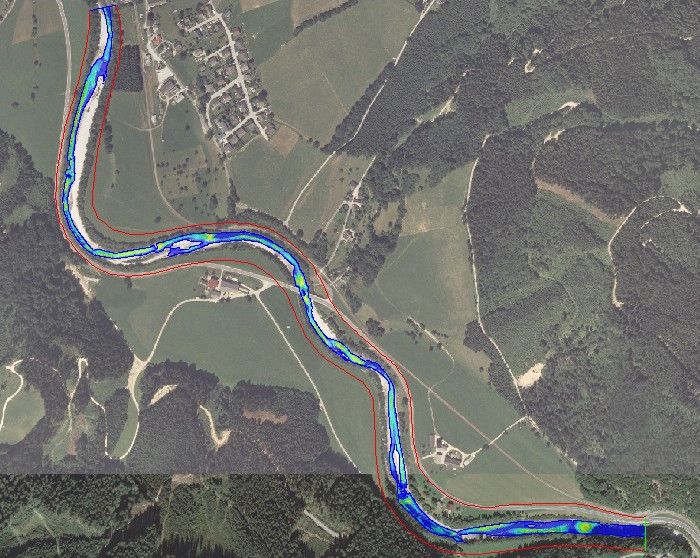
\includegraphics[width=0.56\textwidth,valign=t]{images/0_0035}\\
		& 0+ age class\\
		\multirow{4}{*}{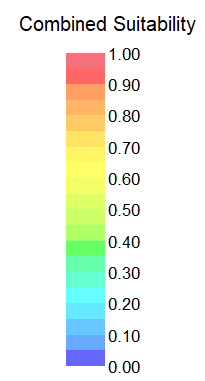
\includegraphics[width=0.3\textwidth,valign=t]{images/suitability_index}}& 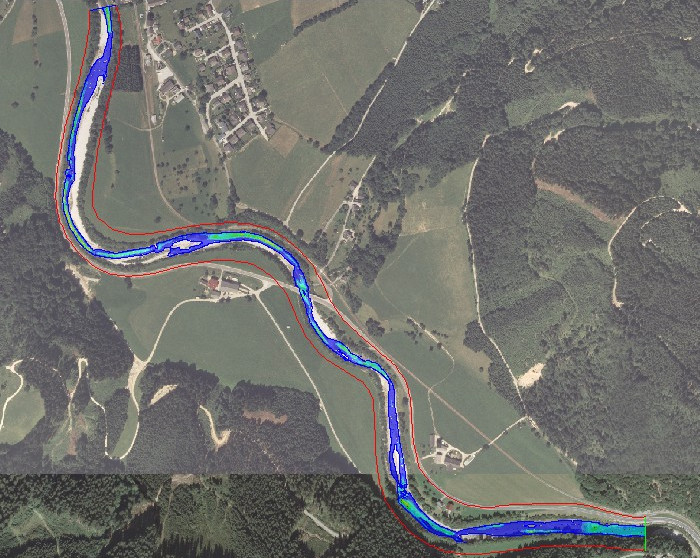
\includegraphics[width=0.56\textwidth,valign=t]{images/1_0035}\\
		& 1+ age class\\
		& 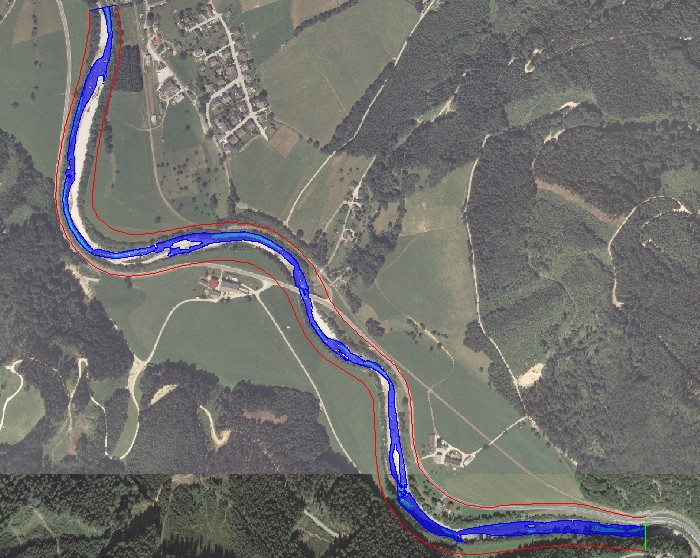
\includegraphics[width=0.56\textwidth,valign=t]{images/2_0035}\\
		& 2+ age class
		
	\end{tabular}
	\label{fig:0035}
	
	\caption{River2d models of the Ybbs river at \SI[per-mode=symbol]{0.35}{\cubic\meter\per\second}.}   %% figure Caption
	
\end{figure}


\newpage                                                                %% End page


%%----------------Appendix B
\fakesubsection{\SI[per-mode=symbol]{2.16}{\cubic\meter\per\second} flow rate models} %% Adds subsection to TOC but not the page
\subsection*{Appendix B}\label{appendixB}                        %% Adds subsection to page but not the TOC

\renewcommand\thefigure{A.\arabic{figure}}                          %% Begins numbering the appendix figures with A
\setcounter{figure}{0}                                              %% Restarts the figure counter

\centering
\begin{figure}[h!]                                                   	%% 00.35 Flow rate
	\begin{tabular}{ l  c }
		
		& 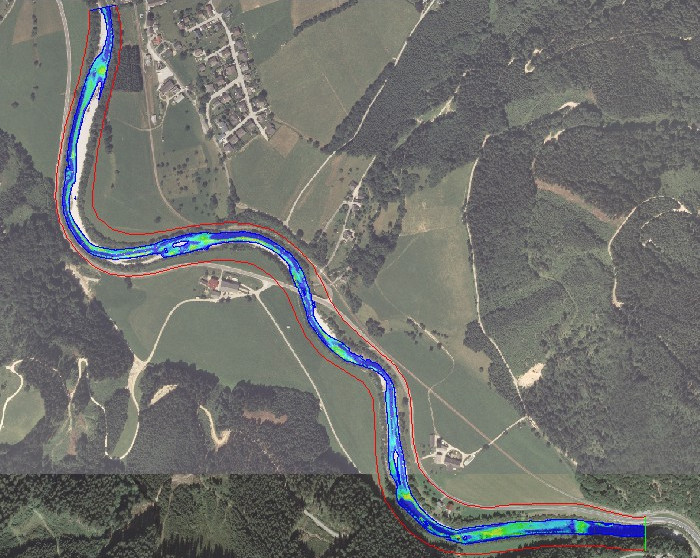
\includegraphics[width=0.56\textwidth,valign=t]{images/0_0216}\\
		& 0+ age class\\
		\multirow{4}{*}{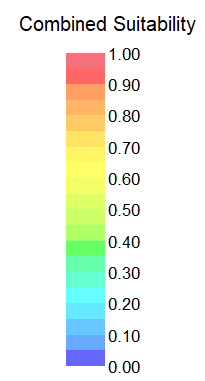
\includegraphics[width=0.3\textwidth,valign=t]{images/suitability_index}}& 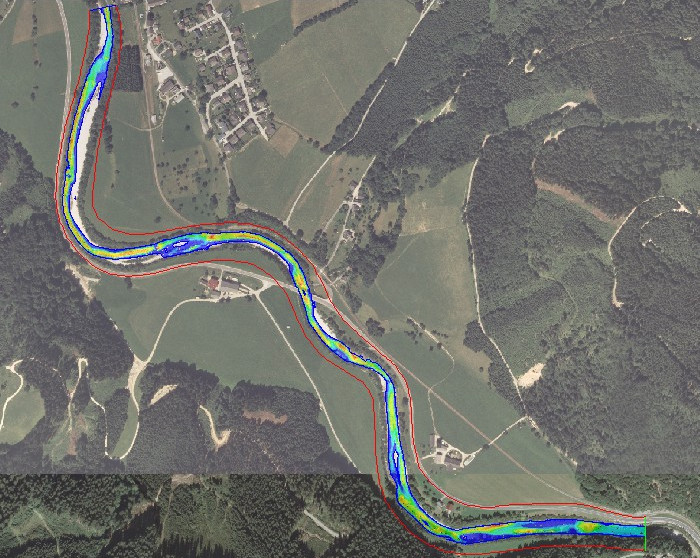
\includegraphics[width=0.56\textwidth,valign=t]{images/1_0216}\\
		& 1+ age class\\
		& 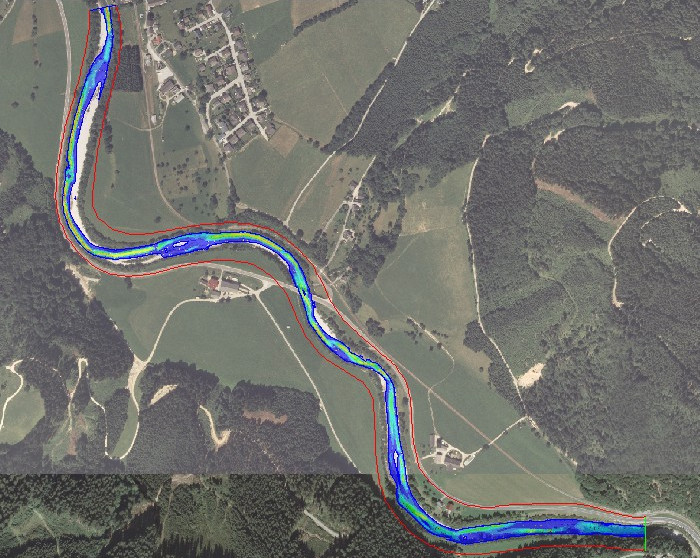
\includegraphics[width=0.56\textwidth,valign=t]{images/2_0216}\\
		& 2+ age class
		
	\end{tabular}
	\label{fig:0216}
	
	\caption{River2d models of the Ybbs river at \SI[per-mode=symbol]{2.16}{\cubic\meter\per\second}.}   %% figure Caption
	
\end{figure}


\newpage                                                                %% End page


%%----------------Appendix C
\fakesubsection{\SI[per-mode=symbol]{6}{\cubic\meter\per\second} flow rate models} %% Adds subsection to TOC but not the page
\subsection*{Appendix C}\label{appendixC}                        %% Adds subsection to page but not the TOC

\renewcommand\thefigure{A.\arabic{figure}}                          %% Begins numbering the appendix figures with A
\setcounter{figure}{0}                                              %% Restarts the figure counter

\centering
\begin{figure}[h!]                                                   	%% 00.35 Flow rate
	\begin{tabular}{ l  c }
		
		& 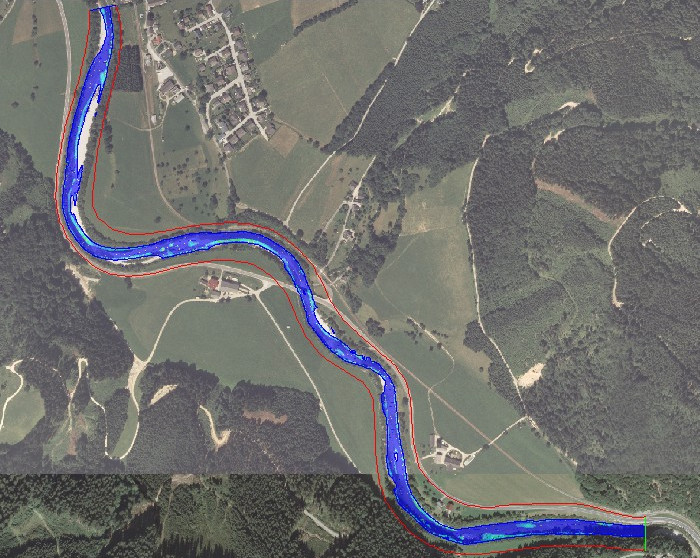
\includegraphics[width=0.56\textwidth,valign=t]{images/0_0600}\\
		& 0+ age class\\
		\multirow{4}{*}{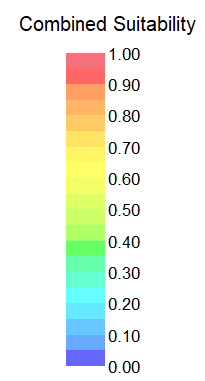
\includegraphics[width=0.3\textwidth,valign=t]{images/suitability_index}}& 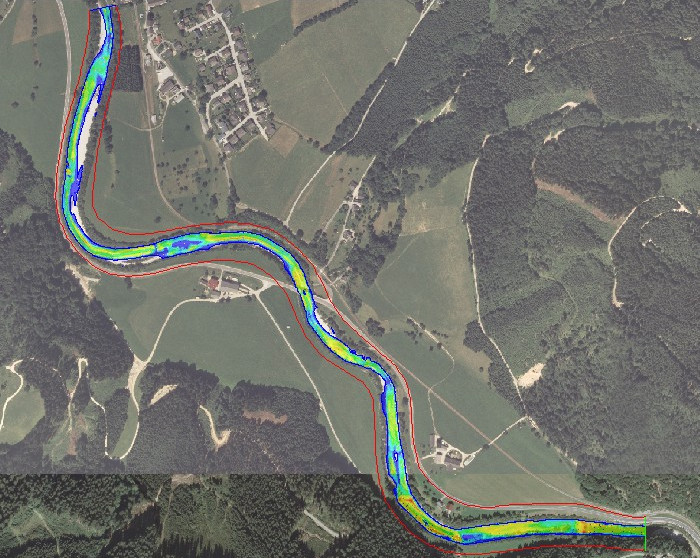
\includegraphics[width=0.56\textwidth,valign=t]{images/1_0600}\\
		& 1+ age class\\
		& 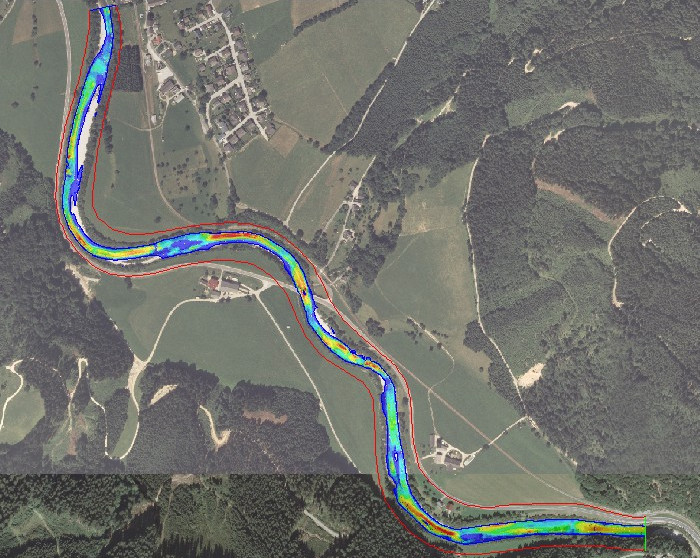
\includegraphics[width=0.56\textwidth,valign=t]{images/2_0600}\\
		& 2+ age class
		
	\end{tabular}
	\label{fig:0600}
	
	\caption{River2d models of the Ybbs river at \SI[per-mode=symbol]{6.00}{\cubic\meter\per\second}.}   %% figure Caption
	
\end{figure}


\newpage                                                                %% End page


%%----------------Appendix D
\fakesubsection{\SI[per-mode=symbol]{13}{\cubic\meter\per\second} flow rate models} %% Adds subsection to TOC but not the page
\subsection*{Appendix D}\label{appendixD}                        %% Adds subsection to page but not the TOC

\renewcommand\thefigure{A.\arabic{figure}}                          %% Begins numbering the appendix figures with A
\setcounter{figure}{0}                                              %% Restarts the figure counter

\centering
\begin{figure}[h!]                                                   	%% 00.35 Flow rate
	\begin{tabular}{ l  c }
		
		& 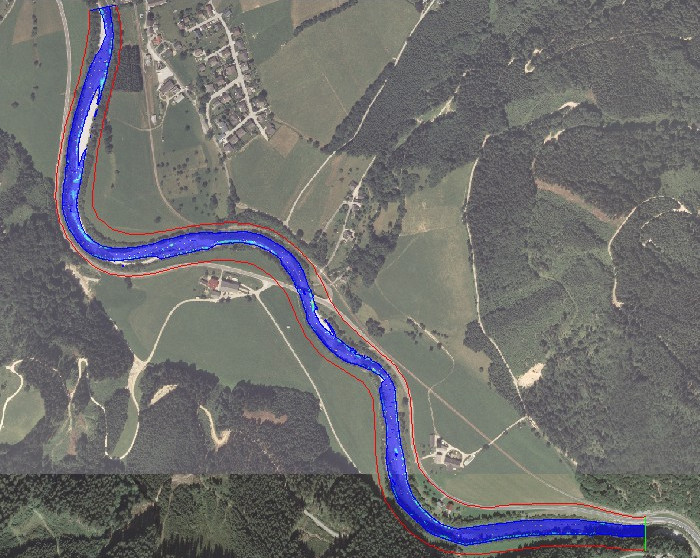
\includegraphics[width=0.56\textwidth,valign=t]{images/0_1300}\\
		& 0+ age class\\
		\multirow{4}{*}{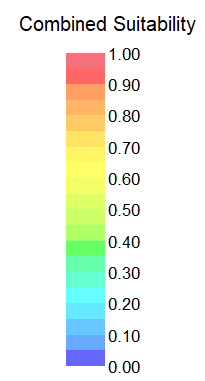
\includegraphics[width=0.3\textwidth,valign=t]{images/suitability_index}}& 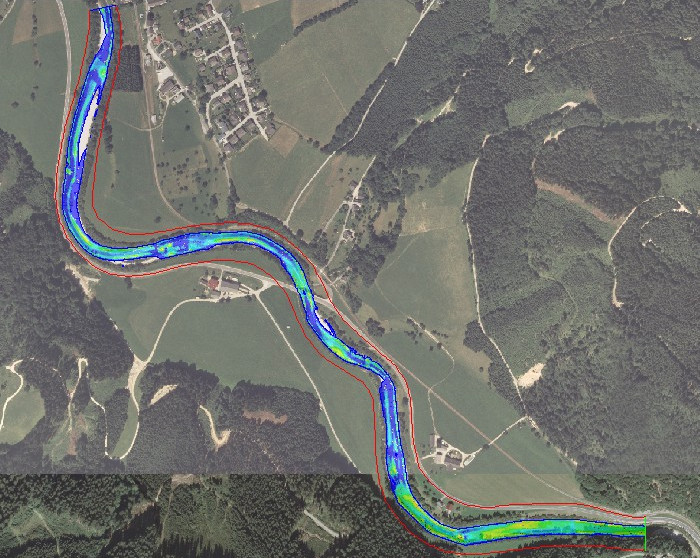
\includegraphics[width=0.56\textwidth,valign=t]{images/1_1300}\\
		& 1+ age class\\
		& 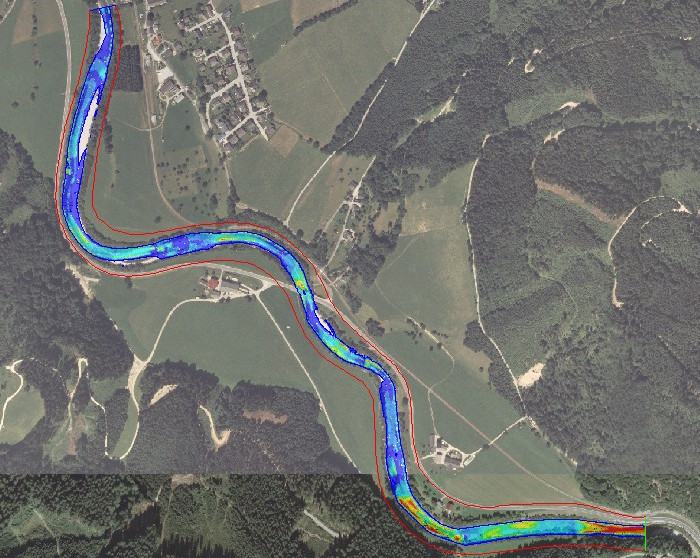
\includegraphics[width=0.56\textwidth,valign=t]{images/2_1300}\\
		& 2+ age class
		
	\end{tabular}
	\label{fig:1300}
	
	\caption{River2d models of the Ybbs river at \SI[per-mode=symbol]{13.00}{\cubic\meter\per\second}.}   %% figure Caption
	
\end{figure}


\newpage                                                                %% End page


%%----------------Appendix E
\fakesubsection{\SI[per-mode=symbol]{20}{\cubic\meter\per\second} flow rate models} %% Adds subsection to TOC but not the page
\subsection*{Appendix E}\label{appendixE}                        %% Adds subsection to page but not the TOC

\renewcommand\thefigure{A.\arabic{figure}}                          %% Begins numbering the appendix figures with A
\setcounter{figure}{0}                                              %% Restarts the figure counter

\centering
\begin{figure}[h!]                                                   	%% 00.35 Flow rate
	\begin{tabular}{ l  c }
		
		& 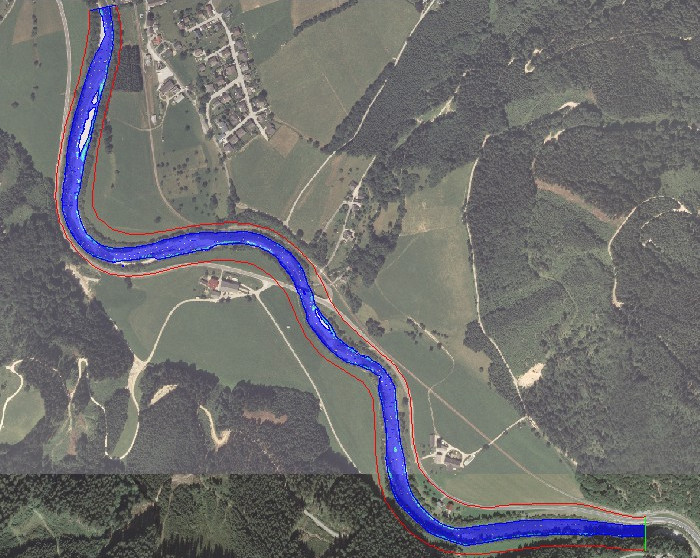
\includegraphics[width=0.56\textwidth,valign=t]{images/0_2000}\\
		& 0+ age class\\
		\multirow{4}{*}{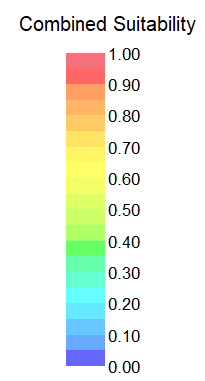
\includegraphics[width=0.3\textwidth,valign=t]{images/suitability_index}}& 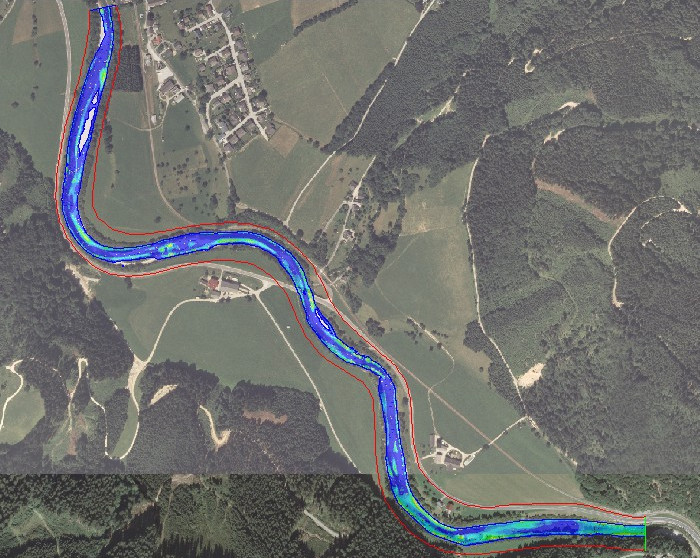
\includegraphics[width=0.56\textwidth,valign=t]{images/1_2000}\\
		& 1+ age class\\
		& 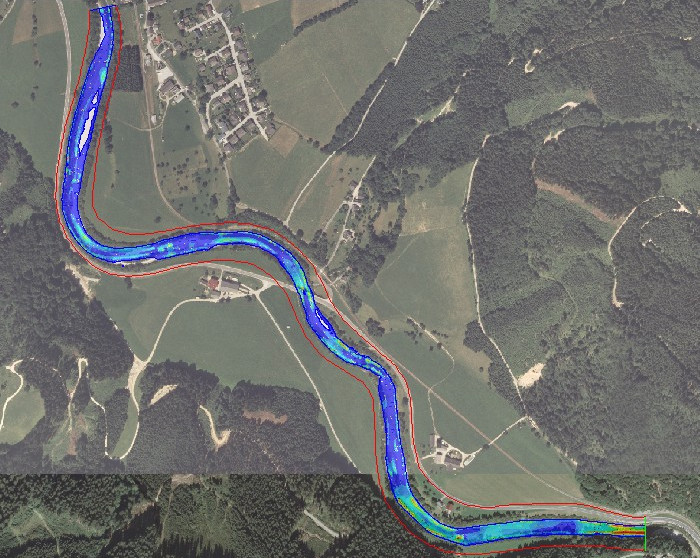
\includegraphics[width=0.56\textwidth,valign=t]{images/2_2000}\\
		& 2+ age class
		
	\end{tabular}
	\label{fig:2000}
	
	\caption{River2d models of the Ybbs river at \SI[per-mode=symbol]{20.00}{\cubic\meter\per\second}.}   %% figure Caption
	
\end{figure}


\newpage                                                                %% End page

                                 %% Clear page and add appendix clear page

\end{document}                              %% End document

